\documentclass[12pt]{article}
\usepackage[utf8]{inputenc}
\usepackage{amssymb}
\usepackage{wasysym}
\usepackage[a4paper, margin=2cm]{geometry}
\usepackage[T1]{fontenc}
\usepackage{CJKutf8}
\usepackage[dvipsnames]{xcolor}
\usepackage{graphicx}
\graphicspath{ {./William Black Exercises/} }
\usepackage{scrextend}
\usepackage{hyperref}
\hypersetup{colorlinks=true,
            linkcolor=blue,
            filecolor=magenta,      
            urlcolor=cyan,}
\urlstyle{same}

\title{\textbf{Proof of Concept - Elaboration II: Testing and Revision}}
\date{08 Oct 2019}
\author{William Black 42920477}
\setlength{\parindent}{0pt}
\setlength{\parskip}{0.5em}

\begin{document}

\underline{\textbf{\Large{Formatting Tests}}}

\section{\large Format any LaTeX section label to be grey and bold.}

\textbf{Intention:} Based on my own new skills in LaTeX, I think I should be able to apply standard formatting to section labels.

\textbf{Action:} In a new sample LaTeX document, applying the normal to the section heading. \vspace{-0.5em}\begin{verbatim}
\section{\textbf{\textcolor{gray}{Section Title Here}}}    \end{verbatim}\vspace{-0.5em}

\textbf{Result:} It works, but leaves the number black. 

\textbf{Action:} Trying it the other way around
\vspace{-0.5em}\begin{verbatim}
\textcolor{gray}{\subsection{\textbf{Section Title Here}}}  \end{verbatim}\vspace{-0.5em}

\textbf{Result:} Test successful. This is good to keep in mind formatting can be applied to only word-count though, as some sections would not be greyed out.

\section{\large Create macro that applies that formatting to all section headings.}

\textbf{Intention:} Use \href{https://en.wikibooks.org/wiki/LaTeX/Creating_Packages}{this tutorial} to make a .cls class or .sty package. The page says "They are very similar, the main difference being that you can load only one class per document." Brian suggests I might make a .sty package, since I'm \textit{not} attempting to make a stylistic rendering of a document.

The instructions then say to write a document preamble to make the macro, and save it in a .sty file.

Using a real essay that I'm currently writing, I'll copy the code for the headings with word counts that I've been typing out by hand so far, and create a file called \texttt{pocgoal.tex} to keep track of the goal. Then I'll write three instructions, one each for sections, subsections, and subsubsections, that applies formatting to two arguments - which will be the heading and the word count separately.

\newpage\textbf{Action:} 

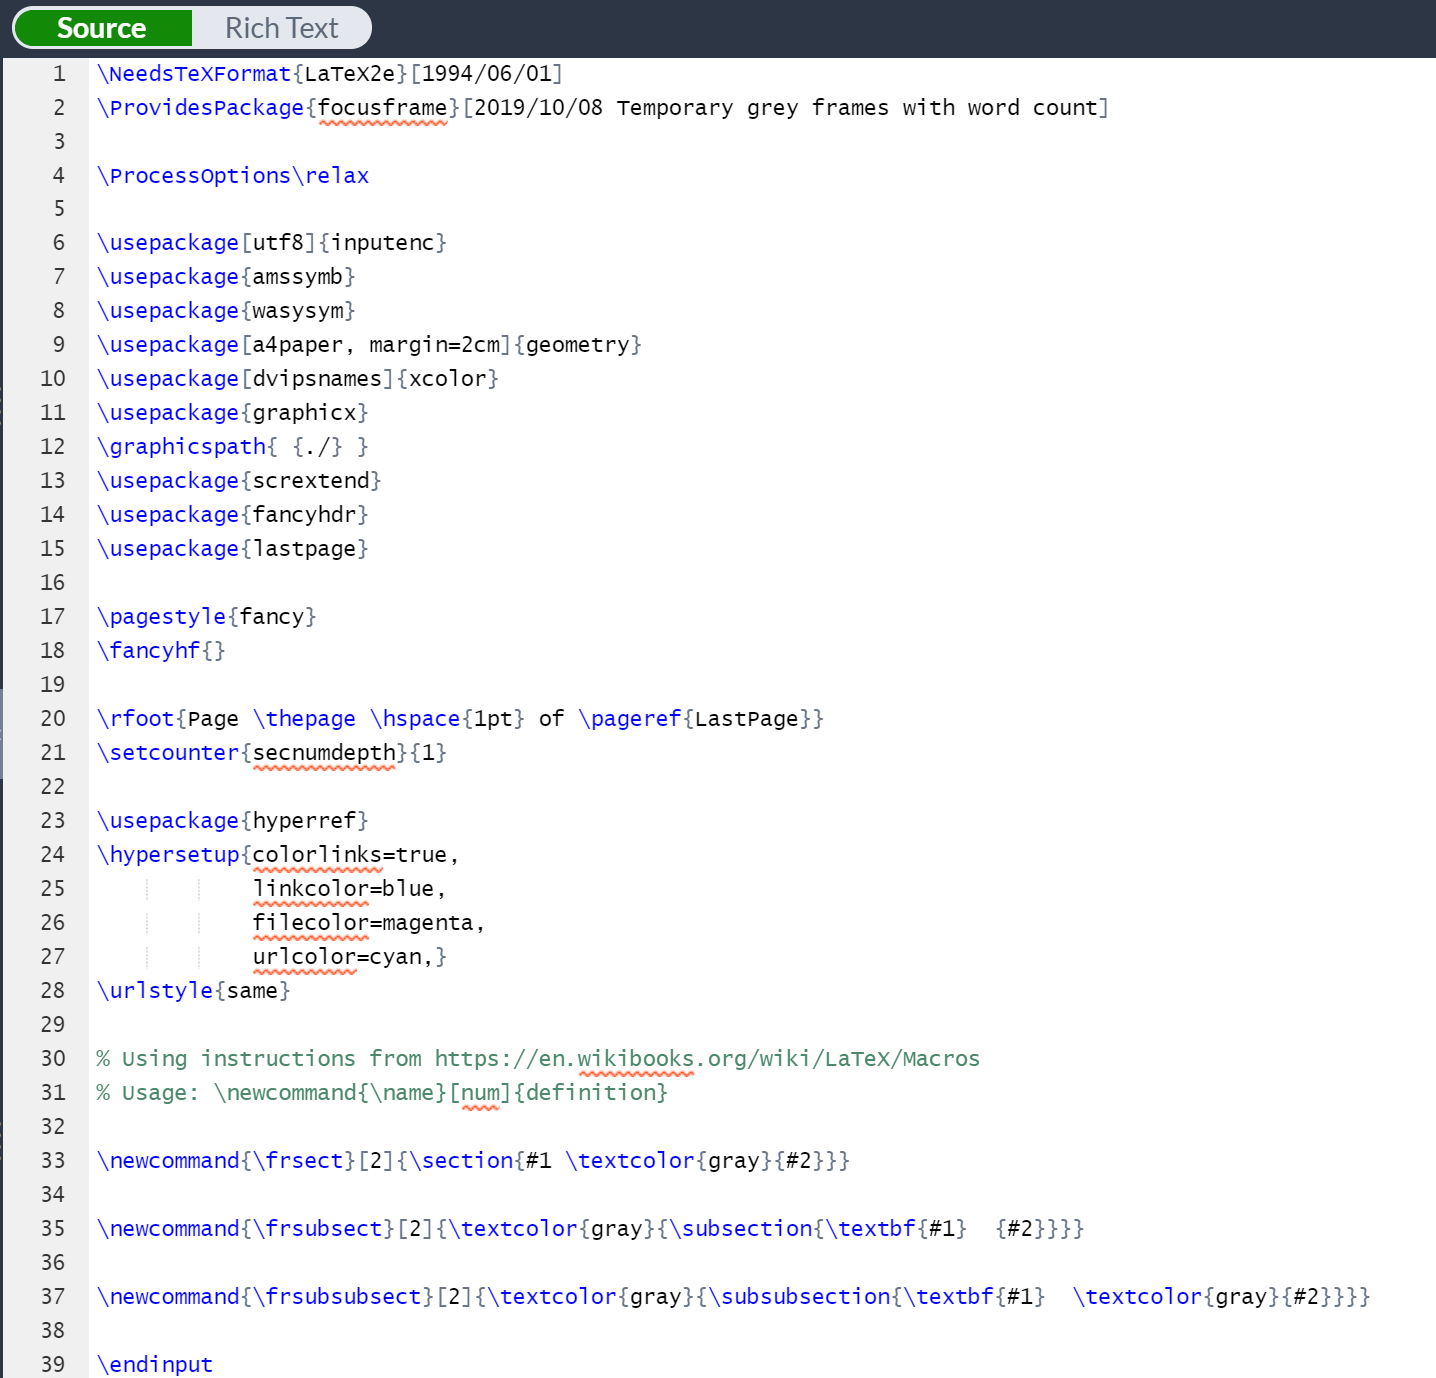
\includegraphics[scale=0.5]{imgfrstyfile.png}

\textbf{Result:} 

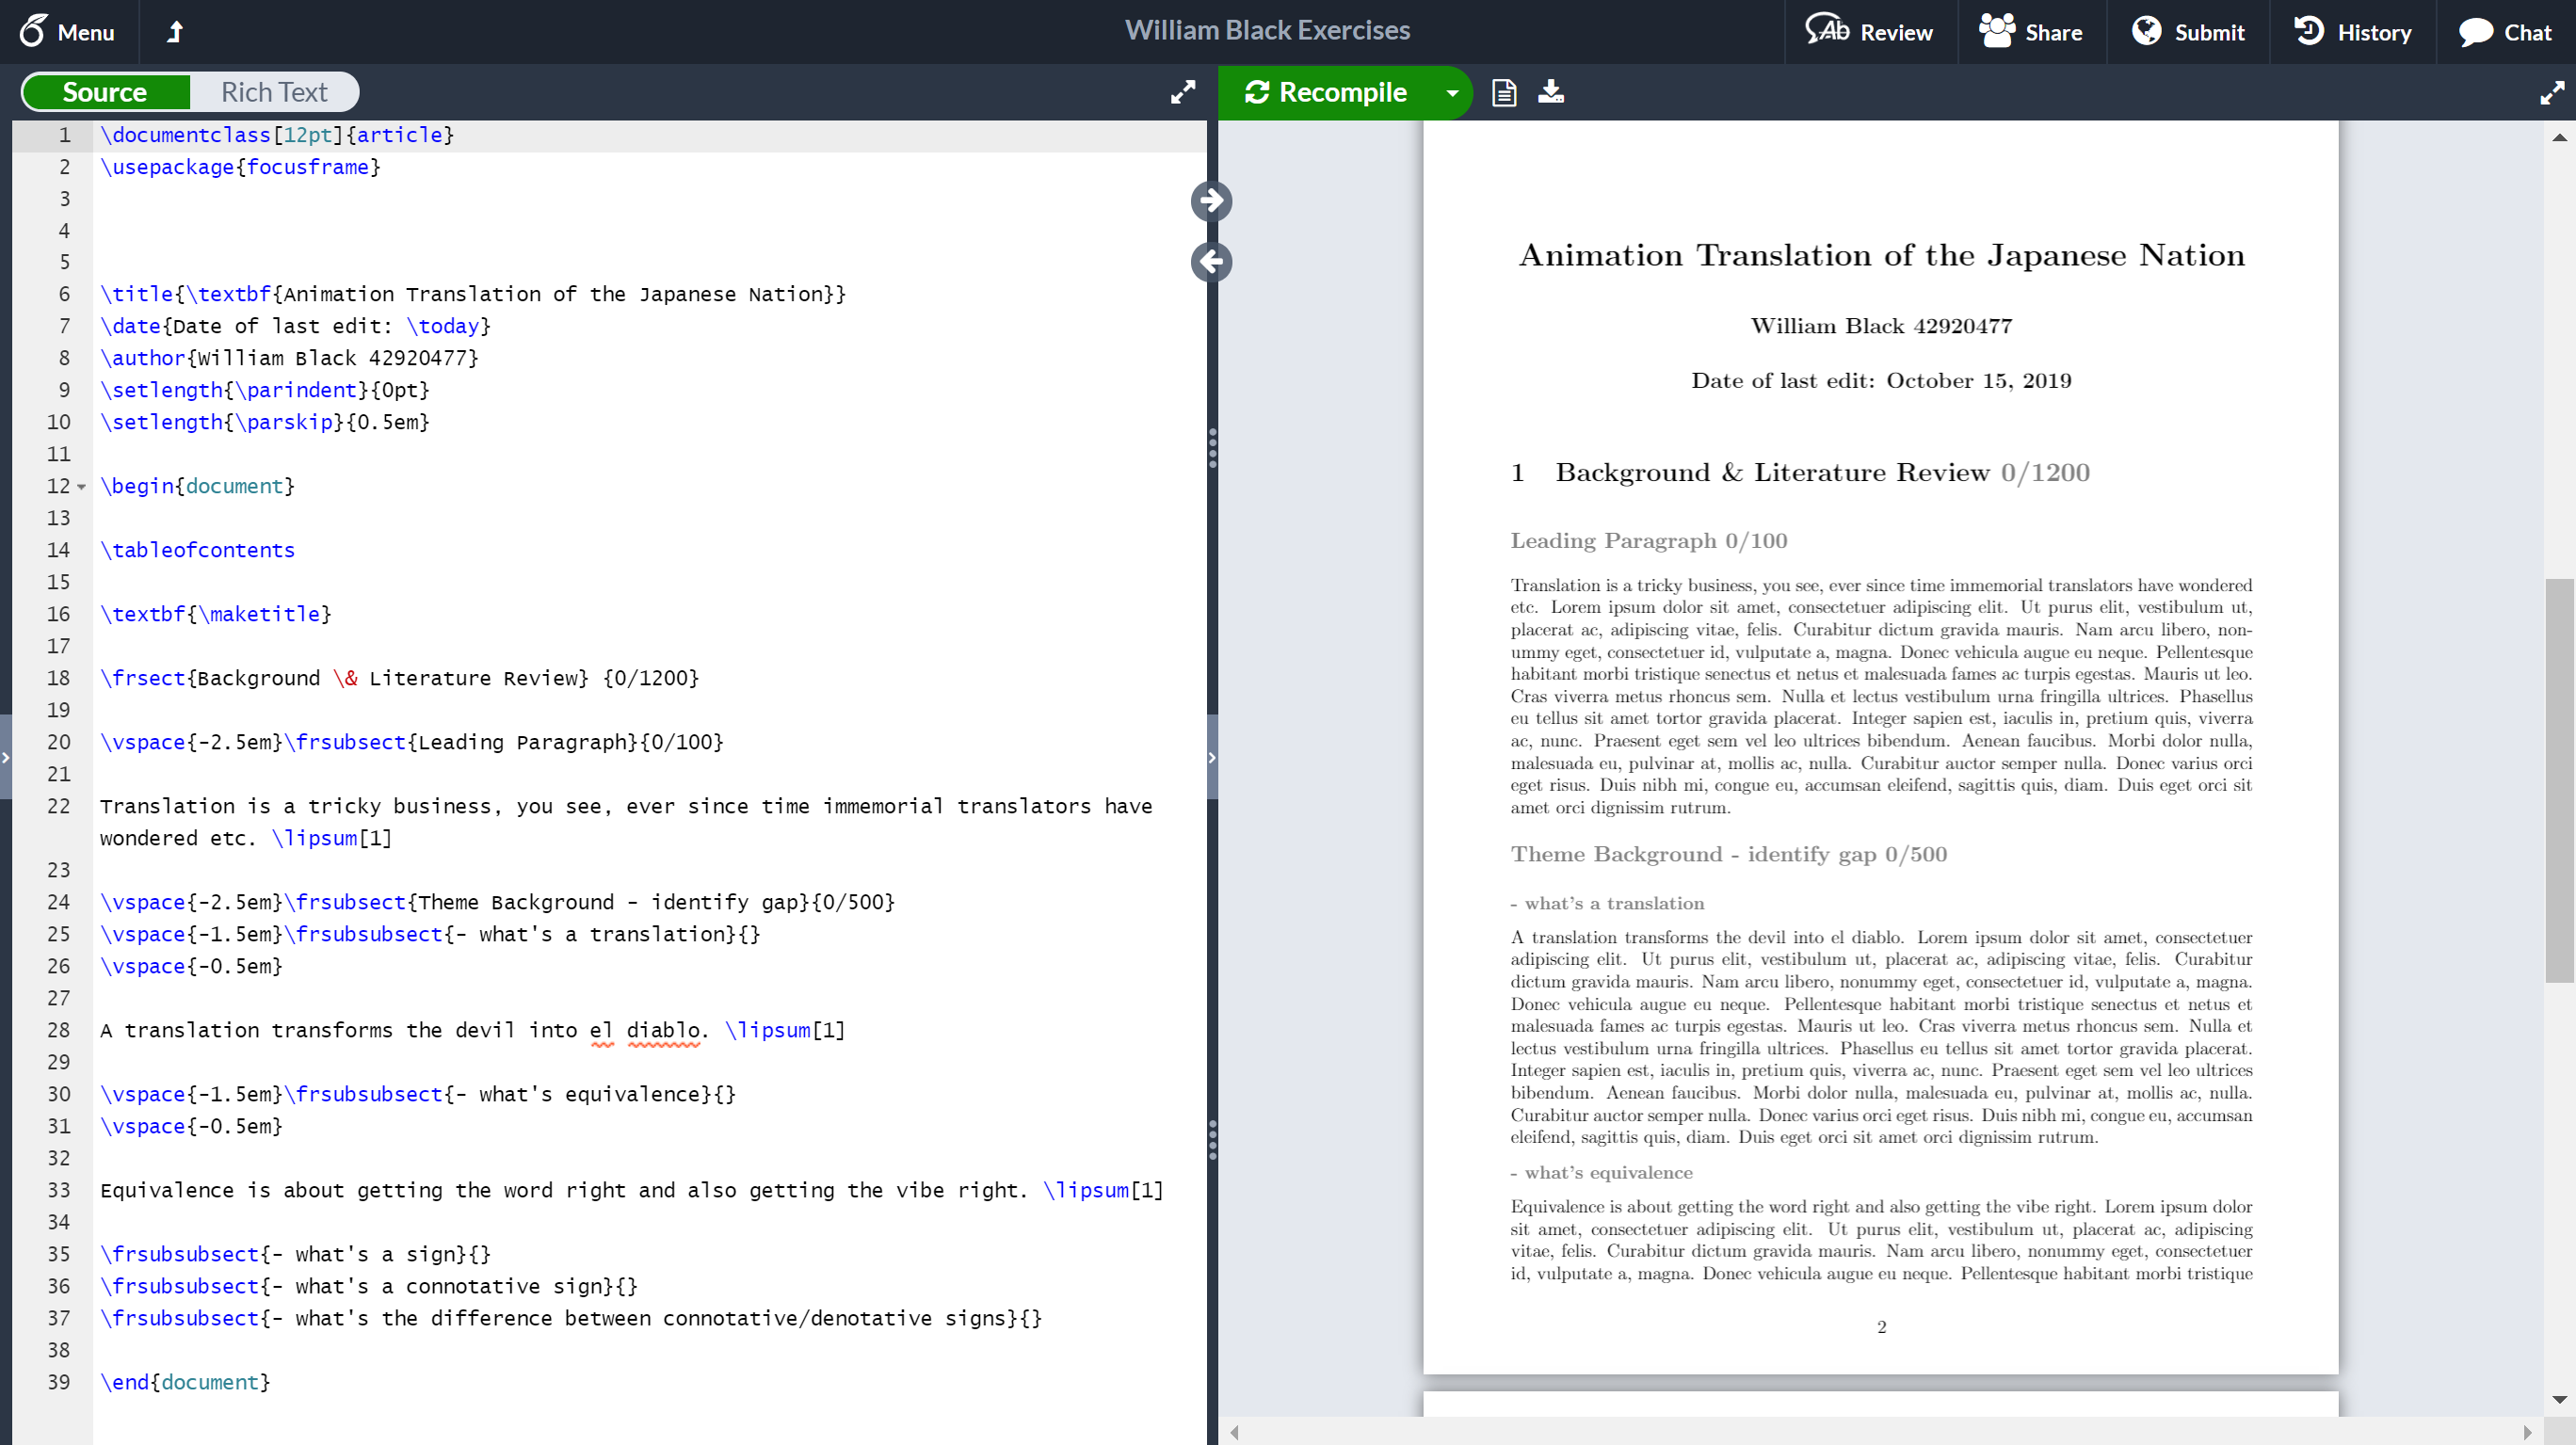
\includegraphics[width=\textwidth]{imgfrvspace.PNG}

The headings and word counts are applying, but I realised I need to change the vertical space to a negative integer to keep a balanced look in the document. It would be easier to add this to the .sty file, as it will always look better with the space I've manually written in.

\newpage\textbf{Action:} 

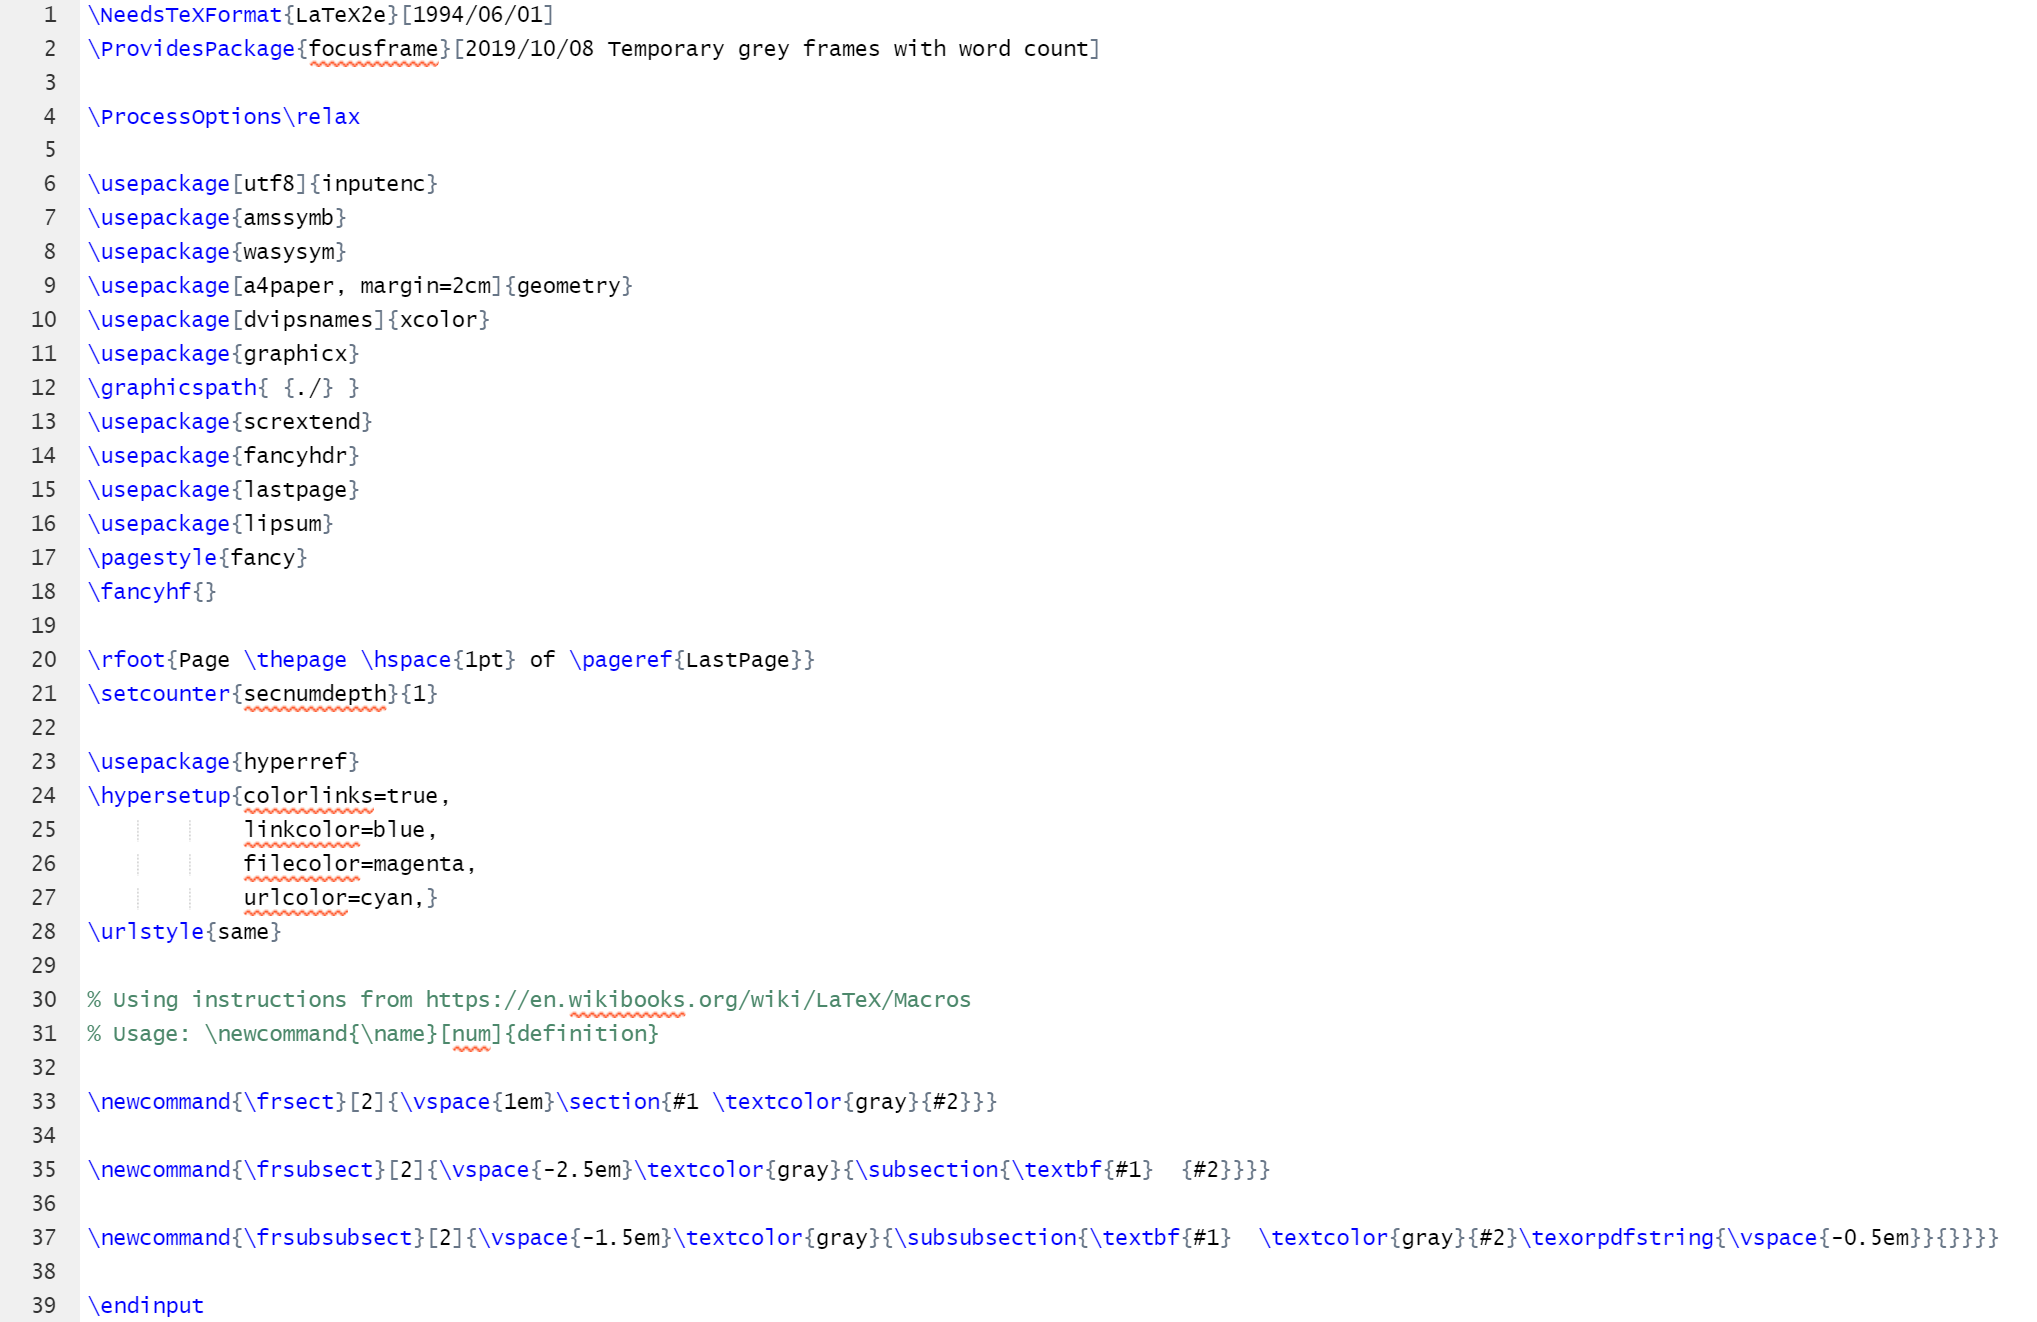
\includegraphics[scale=0.5]{imgfrstyfile2.PNG}

\textbf{Result:} 

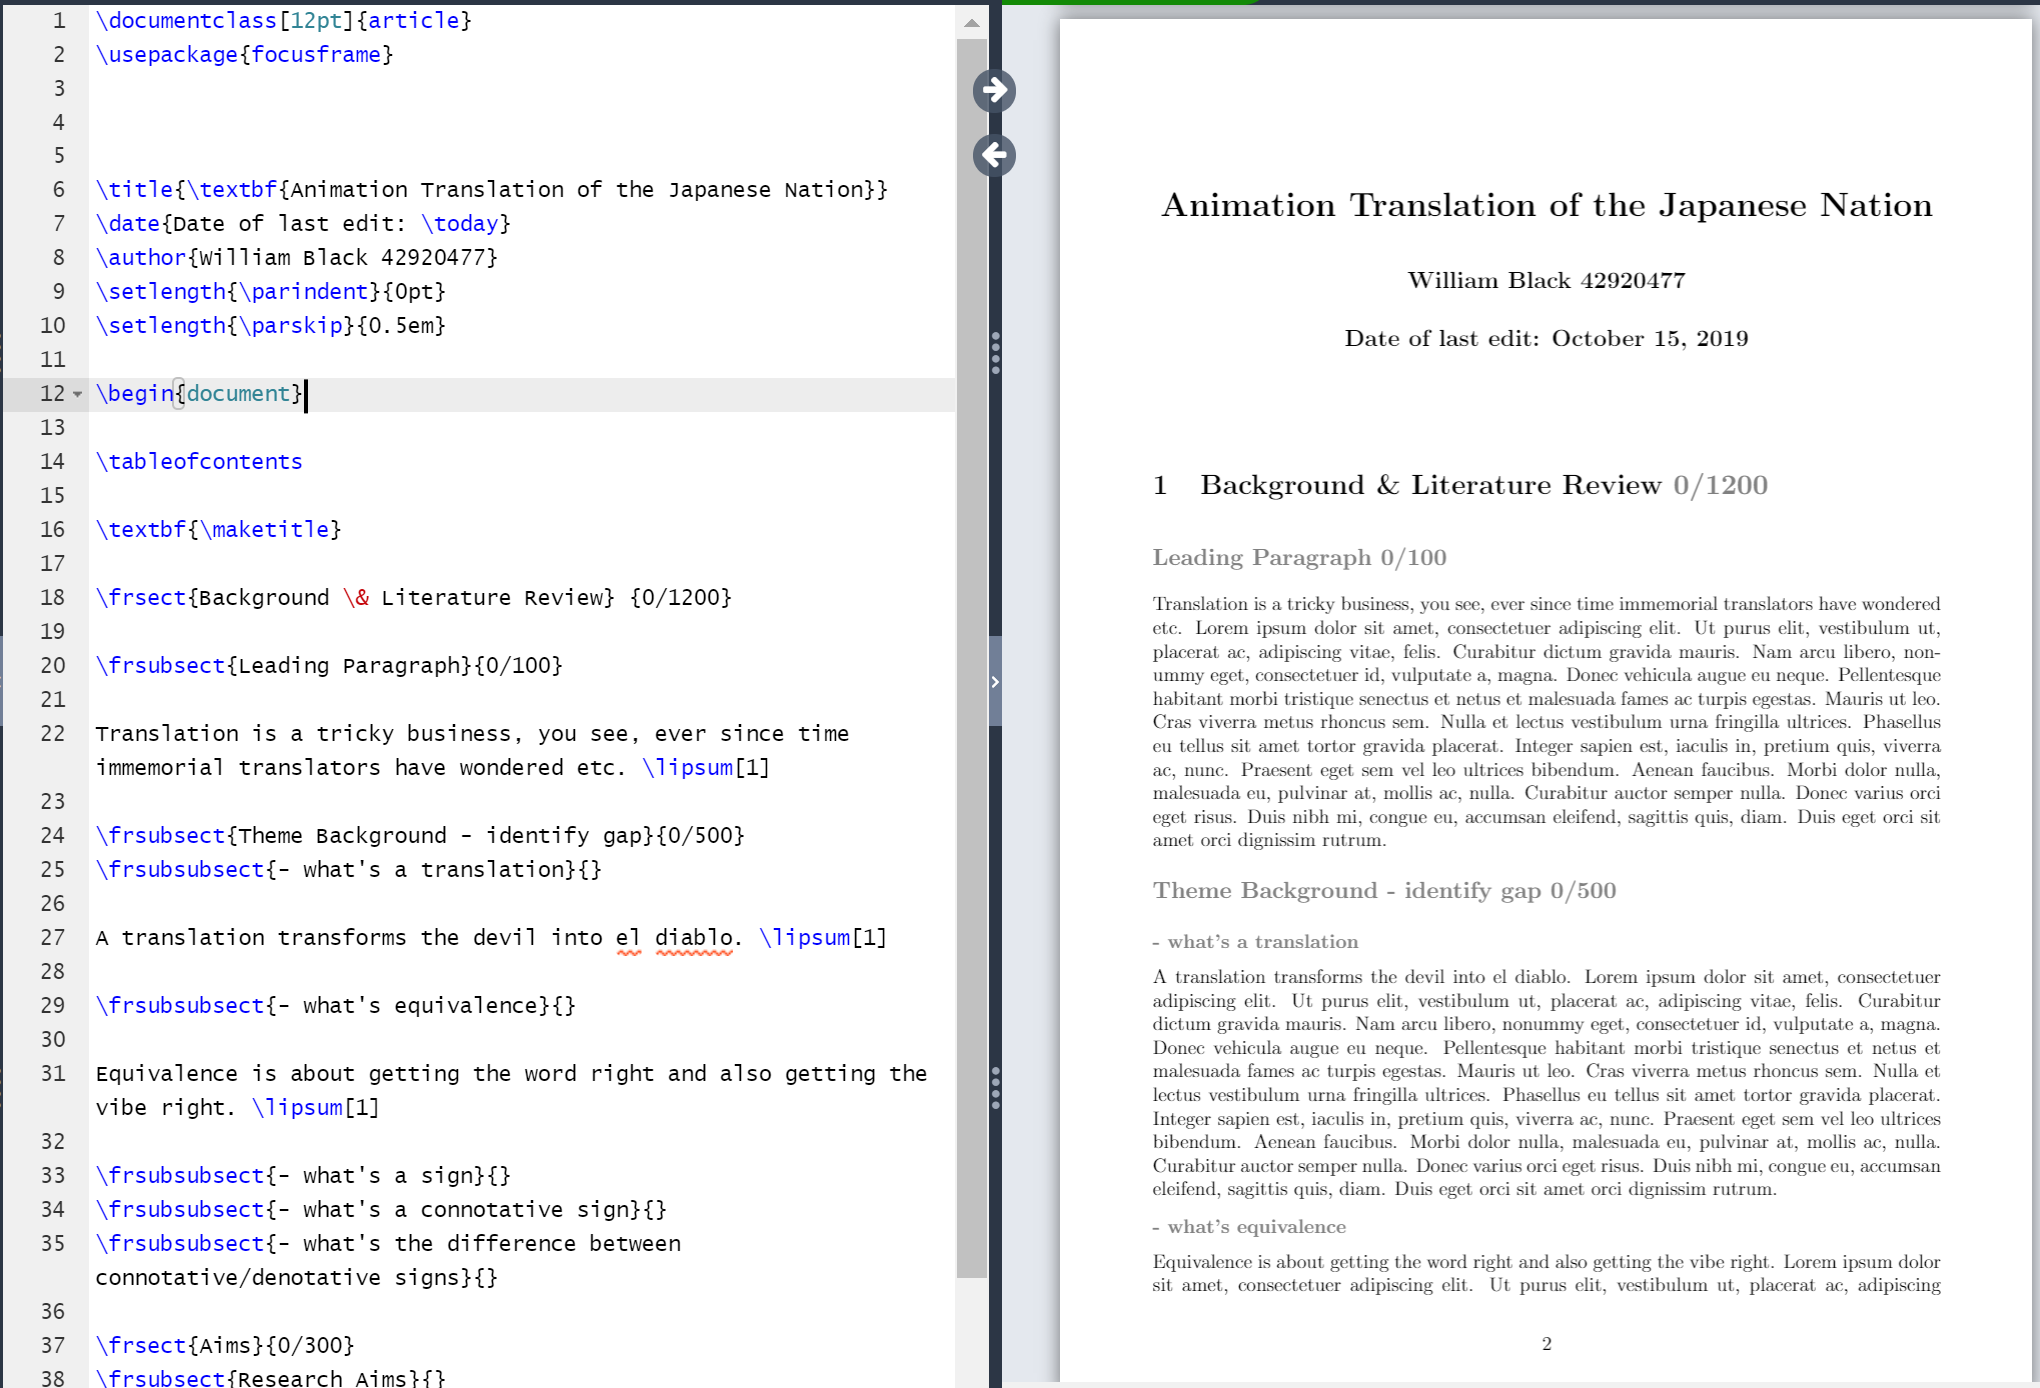
\includegraphics[width=\textwidth]{imgfrvspace2.PNG}

\section{\large Apply macro to all sections, subsections and subsubsections.}

This was inadvertently accomplished during the last test. Formatting was applied by macro, and no longer needs to be applied to sectioning system since the commands already contain sectioning instructions.

\newpage

\underline{\textbf{\Large{Word Count Tests}}}
\section{\large Extract subcount of words in LaTeX}

\textbf{Intention:}
\textbf{Action:}
\textbf{Result:}

There's a \href{https://www.overleaf.com/learn/how-to/Is_there_a_way_to_run_a_word_count_that_doesn\%27t_include_LaTeX_commands\%3F}{word count tool} already built in to Overleaf that excludes LaTeX commands, so at least this is theoretically possible.

There is also a \href{https://app.uio.no/ifi/texcount/}{Perl script} that counts words. A Perl script is a type of programming language that is considered easier to learn than others and works well with UNIX facilities. (Rouse, 2017)

There is also \href{https://tex.stackexchange.com/questions/44618/dynamically-count-and-return-number-of-words-in-a-section}{this tutorial} that implies that extracting a subcount for a specific section is possible through the \texttt{texcount} package.


\section{\large Frames can be toggled on/off} 

Presumably you can just break the code and it stops working, but that doesn't necessarily mean there won't be undesirable consequences like broken code displaying in the document.

One solution might be to add percentage marks to the frames so they become comments and neither function as code nor appear in the document, although this might be annoying to scroll through code and insert them for long documents with dozens of sections. \href{https://vim.fandom.com/wiki/Inserting_text_in_multiple_lines}{Here} is a solution to that where I can apply markers to multiple lines at once, if I choose to use an editor called Vim as my LaTeX editor.

In order to apply \textit{commands} to several parts of a document at once, I may need to create a \href{https://en.wikibooks.org/wiki/LaTeX/Macros}{macro}. It looks like by using \textbackslash newcommand\{\} I will be able to apply any a command to marked points I've prepared in advance throughout the document.

\section{\large Word count is updated with each recompile, turning blue within ten percent of goal, orange within twenty percent of goal, and red when more than thirty percent over.}

It seems like it's at least possible to keep a running count of words in sections that updates with each recompile with a macro, based on an example \href{https://tex.stackexchange.com/a/44626}{seen here}.

LaTeX has an option to use \href{https://en.wikibooks.org/wiki/LaTeX/Macros#Conditionals}{conditionals} with an \texttt{ifthen} package. \href{https://tex.stackexchange.com/questions/13866/why-is-the-ifthen-package-obsolete}{A stackexchange post} talks about this package being obsolete with more modern options being available such as \href{https://ctan.org/pkg/etoolbox}{etoolbox}.

\vspace{1em}
\section*{\underline{\Large{\textbf{Testing:}}}}

\subsection*{Formatting Tests}

After creating a dummy document with lorem ipsum, the first thing to test is applying code to the sectioning system in the first place. The easiest way may be creating a macro. 

\vspace{0.5em}
\underline{Test A: (Testing Duties 1, 2, 3, 6)}

Format any LaTeX section label to be grey and bold.

If this fails, a user-created sectioning system will need to be created to have better control over formatting.

$\downarrow$

\underline{Test B: (Testing Duties 1, 2, 3, 4, 6)}

Create macro that applies that formatting to all section headings.

This might look something roughly like 
\begin{verbatim}
    \newcommand{\framesect}{\section{\insertformattinghere{#1}}}
    \begin{document}
    \framesect{Introduction}
\end{verbatim}

If this fails due to incompatibility with the native sectioning system, a user-created sectioning system may need to be created.

If this fails due to my own weakness of skill, I will need to turn to further resources and guidance supporting macro creation. It may be necessary to follow a completely new route with a different editor, environment, or coding language.

$\downarrow$

\underline{Test C: (Testing Duties 1, 2, 3, 6)}

Apply macro to all labels; sections, subsections, subsubsections.

If this fails, possibly multiple macros will need to be made to cover the different duties required of sections vs subsubsections, for instance, a different macro may need to be created for those sections where the heading is forbidden from being toggled off, and must appear in the final document.

If multiple macros cannot co-exist peacefully or time constraints do not allow completion, a manual solution can be used, for instance, inserting permanent headings after the writing process is finished.

\vspace{2em}
\subsection*{Word Count Tests}

Assuming the formatting tests went smoothly, the process should be mostly repeatable or even extended to the requirements of word counting. If a macro was unable to be created, these tests should still apply to whatever process was used as an alternative.

\underline{Test A: (Testing Duties 1, 2, 3, 4}

Add word count goal to formatting macro.

This should only require one extra element to type at each sectioning label, with an option to not specify word count goal.

If this fails, a separate macro may have to be created.

$\downarrow$

\underline{Test B: (Testing Duties 1, 2, 4)}

Extract a subcount of words for one section using a \texttt{texcount} macro.

If this fails, other macros can be tested.

If all macros fail, a different TeX environment like ConTeXt or LuaTeX may need to be considered, or possibly a different coding language. 

$\downarrow$

\underline{Test C: (Testing Duties 1, 2, 4, 6)}

Test subcount strategy on all levels of sectioning. At each recompile, word counter should be able to return updated results for entire dummy document, each section, each subsection, etc.

If this fails, separate word counts may need to be created to deal with each level of sectioning.

\vspace{2em}
\subsection*{Changing Frame Tests}

Elements of the focus frame are supposed to change automatically and with user input.

\underline{Test A: (Testing Duties 1, 2, 4, 6)}

Extract subcount from section, and where subcount is with ten percent of section word count goal, turn word count from grey to blue using etoolbox.

If no success with etoolbox, other packages like \texttt{ifthen} may be simpler to make, even if not as powerful.

Any solution that passes this test should be replicatable for orange and red counts with their conditions.

\vspace{1em}
\underline{Test B: (Testing Duties 1, 5)}

Create toggle for the macro/process.

This should be the easiest part, it seems that every version of these scripts has an ability to simply say `fframe\=true' somewhere.

If this test fails, a manual solution to turning it off can be found by entering \% marks on coded lines, or simply deleting the code.




\vspace{3em}
\section*{\underline{\textbf{\Large References:}}}

Rouse, M. (2017). What is Perl? - Definition from WhatIs.com. Retrieved 29 August 2019, from https://whatis.techtarget.com/definition/Perl

\end{document}
